\documentclass[english,onecolumn]{IEEEtran}
\usepackage[T1]{fontenc}
\usepackage[latin9]{luainputenc}
\usepackage[letterpaper]{geometry}
\geometry{verbose}
\usepackage{amsfonts}
\usepackage{babel}
\usepackage{ulem}

\usepackage{extarrows}
\usepackage[colorlinks]{hyperref}
\usepackage{listings}
\usepackage{xcolor}
\usepackage[ruled,linesnumbered]{algorithm2e}

\usepackage{amsmath,graphicx}
\usepackage{subfigure} 
\usepackage{cite}
\usepackage{amsthm,amssymb,amsfonts}
\usepackage{textcomp}
\usepackage{bm,pifont}
\usepackage{booktabs}
\usepackage{listings}
\usepackage{xparse}
\usepackage{xcolor}
\definecolor{salmon}{rgb}{1, 0.5020, 0.4471}

\NewDocumentCommand{\codeword}{v}{
\texttt{\textcolor{blue}{#1}}
}

\lstdefinestyle{mystyle}{
    backgroundcolor=\color{backcolour},   
    commentstyle=\color{codegreen},
    keywordstyle=\color{magenta},
    numberstyle=\tiny\color{codegray},
    stringstyle=\color{codepurple},
    basicstyle=\ttfamily\footnotesize,
    breakatwhitespace=false,         
    breaklines=true,                 
    captionpos=b,                    
    keepspaces=true,                 
    numbers=left,                    
    numbersep=5pt,                  
    showspaces=false,                
    showstringspaces=false,
    showtabs=false,                  
    tabsize=2
}

\lstset{style=mystyle}

\providecommand{\U}[1]{\protect\rule{.1in}{.1in}}
\topmargin            -18.0mm
\textheight           226.0mm
\oddsidemargin      -4.0mm
\textwidth            166.0mm
\def\baselinestretch{1.5}


\newtheorem{theorem}{Theorem}[section]
\newtheorem{lemma}[theorem]{Lemma}

\newcommand{\Rbb}{\mathbb{R}}
\newcommand{\Pb}{\mathbf{P}}
\newcommand{\Ib}{\mathbf{I}}
\newcommand{\vb}{\mathbf{v}}
\newcommand{\Ucal}{\mathcal{U}}
\newcommand{\Wcal}{\mathcal{W}}
\newcommand{\Vcal}{\mathcal{V}}
\newcommand{\Rcal}{\mathcal{R}}
\newcommand{\Ncal}{\mathcal{N}}
\newcommand{\bigO}{\mathcal{O}}
\newcommand{\bigS}{\mathcal{S}}
\newcommand{\bA}{{\bf A}}
\newcommand{\bQ}{{\bf Q}}
\newcommand{\bR}{{\bf R}}
\newcommand{\bH}{{\bf H}}
\newcommand{\bU}{{\bf U}}
\newcommand{\bT}{{\bf T}}
\newcommand{\bI}{{\bf I}}
\newcommand{\bq}{{\bf q}}
\newcommand{\bz}{{\bf z}}
\newcommand{\bL}{{\bf L}}
\newcommand{\bx}{{\bf x}}
\newcommand{\bv}{{\bf v}}
\newcommand{\bG}{{\bf G}}
\def\A{\mathbf{A}}
\def\v{\mathbf{v}}

\begin{document}

\begin{center}
	\textbf{\LARGE{SI231 - Matrix Computations, Fall 2020-21}}\\
	{\Large Homework Set \#4}\\
	\texttt{Prof. Yue Qiu and Prof. Ziping Zhao}\\
	\texttt{\textbf{Name:}}   	\texttt{ Tian Yun }  		\hspace{1bp}
	\texttt{\textbf{Major:}}  	\texttt{ Master in CS } 	\\
	\texttt{\textbf{Student No.:}} 	\texttt{ 2019232102}     \hspace{1bp}
	\texttt{\textbf{E-mail:}} 	\texttt{ tianyun@shanghaitech.edu.cn}
\par\end{center}

\noindent
\rule{\linewidth}{0.4pt}
{\bf {\large Acknowledgements:}}
\begin{enumerate}
    \item Deadline: \textcolor{red}{\textbf{2020-11-20 23:59:00}}
    \item Submit your homework at \textbf{Gradescope}.
    Homework \#4 contains two parts, the theoretical part the and the programming part.
    \item About the the theoretical part:
    \begin{enumerate}
            \item[(a)] Submit your homework in \textbf{Homework 4} in gradescope. Make sure that you have correctly select pages for each problem. If not, you probably will get 0 point.
            \item[(b)] Your homework should be uploaded in the \textbf{PDF} format, and the naming format of the file is not specified.
            \item[(c)] No handwritten homework is accepted. You need to use \LaTeX $\,$ in principle.
            \item[(d)] Use the given template and give your solution in English. Solution in Chinese is not allowed. 
        \end{enumerate}
  \item About the programming part:
  \begin{enumerate}
      \item[(a)] Submit your codes in \textbf{Homework 4 Programming part} in gradescope. 
      \item[(b)] When handing in your homework in gradescope, package all your codes into {\sf your\_student\_id+hw4\_code.zip} and upload. In the package, you also need to include a file named {\sf README.txt/md} to clearly identify the function of each file.
     \item[(c)] Make sure that your codes can run and are consistent with your solutions.
  \end{enumerate}
  \item \textbf{Late Policy details can be found in the bulletin board of Blackboard.}
\end{enumerate}
\rule{\linewidth}{0.4pt}

\section*{Study Guide}
\noindent
This homework concerns the following topics:
\begin{itemize}
    \item Eigenvalues, eigenvectors \& eigenspaces 
    \item Algebraic multiplicity \& geometric multiplicity
    \item Eigendecomposition (Eigvenvalue decomposition) \& Eigendecomposition for Hermitian matrices
    \item Similar transformation, Schur decomposition \& 
    Diagonolization
    \item Variational characterizations of eigenvalues
	\item Power iteration \& Inverse iteration
	\item QR iteration \& Hessenberg QR iteration
	\item Givens QR \& Householder QR (from previous lectures)
\end{itemize}


\newpage 
\section{Understanding eigenvalues and Eigenvectors}

\noindent\textbf{Problem 1}. {\color{blue}(6 points + 4 points)}

\noindent
Consider the $2\times 2$ matrix \[ {\bf A} = \begin{bmatrix}
           -4 & -3 \\
            6 & 5
    \end{bmatrix}\,.    \]
\begin{enumerate}
    \item 
    Determine whether $\bA$ can be diagonalized or not. Diagonalize $\bA$ by ${\bf A} = {\bf V}{\bf \Lambda}{\bf V}^{-1}$ if the answer is "yes" or give the reason if the answer is "no".
    
    \item  Give the eigenspace of ${\bf A}$. 
    And then consider: 
    is there a matrix being similar to ${\bf A}$  but have different eigenspaces with it.
    If the answer is "yes", show an example (here you are supposed to give the specific matrix and its eigenspaces), or else explain why the answer is "no" .
\end{enumerate}

{\bf Remarks:} 
\begin{itemize}
    \item In 1), if {\bf A} can be diagonalized, you are supposed to present not only the specific diagonalized matrix but also how do you get the similarity transformation.
    If not, you should give the necessary derivations of the specific reason.
    \item In 2), if your answer is "yes", you are supposed to give the specific matrix and its eigenspaces.
    If "no", you should give the necessary derivations of the specific reason.
\end{itemize}

\noindent
\textbf{Solution.}
\begin{enumerate}
    \item 
    Solution :
    
    $\bA$ can be diagonalized
    
    Assume $|\lambda I - A| = 0$ , $det(\lambda I - A)=(\lambda +4)(\lambda-5)+18 = \lambda^2-\lambda-2=(\lambda-2)(\lambda+1)$
    
    $\lambda_1 = 2,\quad \lambda_2 = -1$
    
    if $\lambda_1 =2$ ,$(2E-A)x = 0$,so the corresponding eignvector will be $\xi_1 = [1 -2]^T$
    
    if $\lambda_1 =-1$ ,$(-E-A)x = 0$,so the corresponding eignvector will be $\xi_1 = [1 -1]^T$
    
    $$
     {\bf V} = \left[\begin{array}{ll}
    	 1 & 1 \\
    	-2 & -1
    \end{array}\right]   
	 {\bf \Lambda} = \left[\begin{array}{ll}
		2 & 0\\
		0 & -1
	\end{array}\right]
$$

$$A = V \Lambda V^{-1}$$

    \item 
\end{enumerate}


\newpage
\noindent\textbf{Problem 2}. \textcolor{blue}{(6 points $\times$ 5)}

\noindent
For a matrix ${\bf A}\in \mathbb{C}^{n\times n}$, 
$\lambda_1, \lambda_2, \ldots, \lambda_n$   are its $n$ eigenvalues 
(though some of them may be the same). 
Prove that:
\begin{enumerate}
    \item The matrix ${\bf A}$ is singular if only if 0 is an eigenvalue of it.
    \item ${\sf rank}({\bf A}) \geq$ number of nonzero eigenvalues of ${\bf A}$.
    \item If ${\bf A}$ admits an  eigendecomposition (eigenvalue decomposition), ${\sf rank}({\bf A}) =$ number of nonzero eigenvalues of ${\bf A}$.
    \item If $\A$ is Hermitian, then all of eigenvalues of $\bA$ are real.
    \item If $\A$ is Hermitian, then eigenvectors corresponding to different eigenvalues are orthogonal.
\end{enumerate}

\noindent
\textbf{Solution}
\begin{enumerate}
    \item $\textbf{Solution}$: 
    
    If 0 is an eigenvalue of $A,$ then $A x=0 \cdot x=0$ for some non-zero $x,$ which clearly means $A$ is singular. On the other hand, if $A$ is singular, then $A x=0$ for some non-zero $x,$ which is to say that $A x=0 \cdot x$ for some non-zero $x$, which obviously means that 0 is an eigenvalue of $A$.
    
    \item     
    $\textbf{Proof}$: 
    
	If a matrix $A$ is diagonalizable, then the algebraic multiplicity of any eigenvalue of $A$ is equal to its geometric multiplicity. In particular, if $A$ is symmetric (Hermitian) or all the eigenvalues of $A$ are distinct, then $A$ is diagonalizable. From rank-nullity theorem, it is known that
	$$
	\operatorname{rank}(A)+\text { nullity }(A)=\operatorname{dim}(A)
	$$
	Nullity is the dimension of the kernel space of $A$. Meaning the number of linearly independent eigenvectors $x$ for which $A x=0 \cdot x .$ So nullity in this case implies the multiplicity of 0 as an eigenvalue of $A$ and hence rank implies the number of nonzero eigenvalues of $A$.
    \item$\textbf{Proof}$: 
    
    *************************************************************************************
    
    Proposition. If $A$ is $n \times m$ and $B$ is $m \times k,$ then
    $$
    \operatorname{rank}(\mathbf{A B}) \leq \min (\operatorname{rank}(\mathbf{A}), \operatorname{rank}(\boldsymbol{B}))
    $$
    since $(A B)_{j, l}=\sum_{v=1}^{n} A_{j, v} B_{v, l},$ the rows of $A B$ are linear combinations of the rows of $B $ that is ${R}(A B) \subseteq {R}(B),$ whence $\operatorname{rank}(A B) \leq \operatorname{rank}(B) .$ Also, $G(A B) \subseteq G(A),$ whence $\operatorname{rank}(A B) \leq \operatorname{rank}(A)$
    
    *************************************************************************************
    
    
    ${\bf A}$ admits an  eigendecomposition (eigenvalue decomposition).We write $A,$ in spectral form $A=V \Lambda V^{-1},$ ; our goal is to show that $\operatorname{rank}(A)=\operatorname{rank}(\Lambda)$
    rank $(A) \leq \operatorname{rank}(V \Lambda) \leq \operatorname{rank}(\Lambda) .$ And since $\Lambda=V^{-1} A V,$ we have also $\operatorname{rank}(\Lambda) \leq \operatorname{rank}\left(V^{-1} A \right) \leq \operatorname{rank}(A)$, so rank(A) = rank($\Lambda$)
    

    
    ${\sf rank}({\bf A})$ = number of nonzero eigenvalues of ${\Lambda}$ = number of nonzero eigenvalues of ${\bf A}$
    \item $\textbf{Proof}$: 
    
    Let $A$ be a Hermitian matrix.
    Then, by definition, $\mathbf{A}=\mathbf{A}^{\dagger},$ where $^{\dagger}$ designates the conjugate transpose.
    Let $\lambda$ be an eigenvalue of $\mathbf{A}$.
    Let $\mathbf{v}$ be an eigenvector corresponding to the eigenvalue $\lambda$ of $\mathbf{A}$.
    Denote with $\langle\cdot, \cdot\rangle$ the inner product on $\mathrm{C}$.
    $$
    \lambda *\langle v, v\rangle=\langle\lambda * v, v\rangle \quad \text { Properties of Complex Inner Product }
    $$
    Definition of Eigenvector: $\lambda * v=\mathbf{A} * v$
    $$
    =\langle v, \mathbf{A} * v\rangle
    $$
    $\mathbf{A}$ is Hermitian, so $\mathbf{A}^{\dagger}=\mathbf{A}$
    $$
    \begin{array}{ll}
    	=\langle v, \lambda * v\rangle & \text { Definition of Eigenvector: } \lambda * v=\mathbf{A} * v \\
    	=\bar{\lambda} *\langle v, v\rangle & \text { Properties of Complex Inner Product }
    \end{array}
    $$
    We have that $v \neq 0,$ and because of the positive definiteness, it must be that:
    $$
    \langle v, v\rangle \neq 0
    $$
    Thus:
    $$
    \langle v, v\rangle \neq 0
    $$
    So we can divide both sides by $\langle v, v\rangle$
    Thus $\lambda=\bar{\lambda}$.
    By Complex Number equals Conjugate iff Wholly Real, $\lambda$ is a real number.
    $\lambda$ was arbitrary, so it follows that every eigenvalue is a real number.
    Hence the result.
    \item $\textbf{Proof}$: 
    
    Suppose that $A u=\lambda u$ and $A v=\mu v$ for $\lambda \neq \mu .$ Then
    $$
    \begin{array}{c}
    	\lambda\langle u, v\rangle=\langle A u, v\rangle=\langle u, A v\rangle=\langle u, \mu v\rangle=\mu\langle u, v\rangle \\
    	66
    \end{array}
    $$
    since $\mu \neq \lambda$ it follows that $\langle u, v\rangle=0$. Suppose that $A$ has $n$ distinct eigenvalues $\left\{\lambda_{1}, \ldots, \lambda_{n}\right\}$ with corresponding orthogonal
    eigenvectors $\left\{u_{1}, \ldots, u_{n}\right\} .$ Let us also agree to scale the eigenvectors so that
    $$
    \left\langle u_{i}, u_{j}\right\rangle=\delta_{i j}
    $$
    where $\delta_{i j}$ is the so-called Kronecker delta
    $$
    \delta_{i j}=\left\{\begin{array}{ll}
    	0 & \text { if } i \neq j \\
    	1 & \text { if } i=j
    \end{array}\right.
    $$
    We recall that the eigenvalue equation can be written in matrix form
    $$
    A U=U \Lambda
    $$
    where $U=\left(u_{1} u_{2} \ldots u_{n}\right)$ and $\Lambda=\operatorname{diag}\left\{\lambda_{1}, \ldots, \lambda_{n}\right\} .$ We now observe from the orthonor-
    mality of the eigenvectors that
    $$
    U^{*} U=I
    $$
    Hence $U^{-1}=U^{*}$ and consequently
    $$
    A=U \Lambda U^{*}
    $$
    In other words, $A$ can be diagonalized in a particularly simple way.
\end{enumerate}

\clearpage
\section{Understanding The Eigenvalues of Real Symmetric Matrices}
\noindent\textbf{Problem 3}. \textcolor{blue}{(12 points)}
\noindent 
Let $\bA\in \Rbb^{n\times n}$ be a symmetric matrix, $\bigS_k$ denote a subspace of $\Rbb^n$ of dimension $k$, and $\lambda_1\geq \lambda_2\geq...\geq \lambda_n$ represent the eigenvalues of $\bA$. 
For any $k\in\{1,2,3,...,n\}$, prove that \[\lambda_k=\min\limits_{\bigS_{n-k+1}\subseteq \Rbb^n}\max\limits_{\bx\in\bigS_{n-k+1},||\bx||_2=1} \bx^T\bA\bx.\]

\noindent
\textbf{Solution.}

Let $A=Q^{T} \Lambda Q$ be the eigendecomposition of $A . \quad$ We observe that $x^{T} A x=x^{T} Q^{T} \Lambda Q x=$ $(Q x)^{T} \Lambda(Q x),$ and since $Q$ is orthogonal, $\|Q x\|=\|x\| .$ Thus it suffices to consider the case when $A=\Lambda$ is a diagonal matrix with the eigenvalues $\lambda_{1}, \ldots, \lambda_{n}$ in the diagonal. Then we can write
$$
x^{T} A x=\left(\begin{array}{lll}
	x_{1} & \cdots & x_{n}
\end{array}\right)\left(\begin{array}{lll}
	\lambda_{1} & & \\
	& \ddots & \\
	& & \lambda_{n}
\end{array}\right)\left(\begin{array}{c}
	x_{1} \\
	\vdots \\
	x_{n}
\end{array}\right)=\sum_{i=1}^{n} \lambda_{i} x_{i}^{2}
$$
We note that when $A$ is diagonal, the eigenvectors of $A$ are $v_{k}=e_{k},$ the standard basis vector in $\mathbb{R}^{n},$ i.e. $\left(e_{k}\right)_{i}=1$ if $i=k,$ and $\left(e_{k}\right)_{i}=0$ otherwise. Then the condition $x \in S_{k-1}^{\perp}$ implies $x \perp e_{i}$ for $i=1, \ldots, k-1$ so $x_{i}=\left\langle x, e_{i}\right\rangle=0 .$ Therefore, for $x \in S_{k-1}^{\perp}$ with $\|x\|=1,$ we have
$$
x^{T} A x=\sum_{i=1}^{n} \lambda_{i} x_{i}^{2}=\sum_{i=k}^{n} \lambda_{i} x_{i}^{2} \geq \lambda_{k} \sum_{i=k}^{n} x_{i}^{2}=\lambda_{k}\|x\|^{2}=\lambda_{k}
$$
On the other hand, plugging in $x=e_{k} \in S_{k-1}^{\perp}$ yields $x^{T} A x=\left(e_{k}\right)^{T} A e_{k}=\lambda_{k} .$ This shows that
$$
\lambda_{k}=\min _{\|x\|=1 \atop x \in S_{h-1}^{\perp}} x^{T} A x
$$
Similarly, for $\mid x \|=1$
$$
x^{T} A x=\sum_{i=1}^{n} \lambda_{i} x_{i}^{2} \leq \lambda_{\max } \sum_{i=1}^{n} x_{i}^{2}=\lambda_{\max }\|x\|^{2}=\lambda_{\max }
$$
On the other hand, taking $x=e_{n}$ yields $x^{T} A x=\left(e_{n}\right)^{T} A e_{n}=\lambda_{\max } .$ Hence we conclude that
$$
\lambda_{\max }=\max _{\|x\|=1} x^{T} A x
$$
\newpage
\noindent\textbf{Problem 4}. \textcolor{blue}{(5 points+8 points+10 points)}
\noindent To assist the understanding of this problem, we first provide some \textbf{basic concepts of graph theory:}
 
\ding{172} A \textit{simple graph} $G$ is a pair $(V,E)$, such that
\begin{itemize}
	\item 
	$V$ is the set of vertices;
	
	\item 
	$E$ is the set of edges and every edge is denoted by an \textit{unordered} pair of its two \textit{distinct} vertices.
\end{itemize}


\ding{173} If $i,j$ are two distinct vertices and $(i,j)$ is an edge, we then say that $i$ and $j$ are \textit{adjacent}. A graph is called $d$-regular graph if every vertex in the graph is adjacent to $d$ vertices, where $d$ is a positive integer.

\ding{174} Given two graphs $G_1=(V_1,E_1)$ and $G_2=(V_2,E_2)$, if $V_1\subset V_2$ and $E_1\subset E_2$, we call $G_1$ the \textit{subgraph} of $G_2$. 
Furthermore,  we call $G_1$ the \textit{connected component} of $G_2$ 
if 
\begin{itemize}
    \item 
	any vertex in $G_1$ is only connected to vertices in $G_1$.
	\item 
	any two vertices in $G_1$ are connected either directly or via some other vertices in $G_1$;
\end{itemize}
\vspace{3mm}
\noindent 
Suppose $G=(V,E)$ is a simple graph with $n$ vertices indexed by $1,2,...,n$ respectively. 
The adjacency matrix of $G$ is a matrix $\bA\in \Rbb^{n\times n}$ given by

\begin{equation}
\bA_{i,j}=\left\{
\begin{aligned}
1 &, \text{ if vertex } i \text{ and vertex } j \text{ are adjacent;}\\
0 &, \text{ otherwise.}
\end{aligned}
\right.
\end{equation}
Besides, if $G$ is a $d$-regular graph, its \textit{normalized Laplacian matrix} $\bL$ is defined as $\bL\triangleq \bI-\frac{1}{d}\bA$, where $\bI$ is the identity matrix. 
Let $\lambda_1\geq \lambda_2\geq...\geq \lambda_n$ denote the eigenvalues of $\bL$. 
Please prove the following propositions:
\begin{enumerate}
    \item For any vector $\bx \in \Rbb^n$, it follows that 
	\begin{equation}
	\label{C1+}
		\bx^T\bL\bx=\frac{1}{d}\sum_{(i,j)\in E}(\bx_i-\bx_j)^2,
	\end{equation} 
	where $i,j$ represent two distinct vertices and $(i,j)\in E$ represents an edge between $i$ and $j$ in the graph $G$.
	\item $\lambda_n=0$ and $\lambda_1\leq 2$.
	\item {\color{blue}(\textbf{Bonus Problem)}} the graph $G$ has at least $(n-k+1)$ connected components if and only if $\lambda_k=0$. 
\end{enumerate}



\noindent\textbf{Hint:} 
The matrix $\bL$ is real and symmetric. 
	You can directly utilize Courant-Fischer Theorem without proof. Particularly, you may need to utilize the min-max form of the Courant-Fischer Theorem for the Bonus Problem.


\noindent
\textbf{Solution}
\begin{enumerate}
    \item Insert your solution here ...
    \item
    \item
\end{enumerate}

%%%%%%%%%%%%%%%%%%%%%%%%%%%%%%%%%%%%%%%%%%%%%%%%%%%%%%%%%%%%%%%%%%%%%%
%%%%%%%%%%%%%%%%%%%%%%%%%%%%%%%%%%%%%%%%%%%%%%%%%%%%%%%%%%%%%%%%%%%%%%

\newpage

\section{Eigenvalue Computations}
\subsection{Power Iteration} 
\noindent
\textbf{Problem 5.}
\textcolor{blue}{(20 points)}

Consider the $2\times 2$ matrix $\bA$
\[
\bA = \begin{bmatrix}
	0 & \alpha \\
	\beta & 0
\end{bmatrix}\,,\quad \text{ with }\alpha,\beta > 0\,.
\]
\begin{enumerate}
    \item Find the eigenvalues and eigenvectors of $\bA$ by hand. \textcolor{blue}{(5 points)}
    \item Program \textbf{the power iteration} (See Algorithm \ref{alg:power_iter}) and \textbf{the inverse iteration} (See Algroithm \ref{alg:inverse_iter}) respectively and report the output of two algorithms for $\bA$ (you can determine $\alpha,\beta$ by yourself), do the two algorithms converge or not? Report what you have found (you can use plots to support your analysis). \textcolor{blue}{(10 points: programming takes 5 points and the analysis takes 5 points)}
    After a few iterations, the sequence given by the power iteration fails to converge, explain why. \textcolor{blue}{(5 points)}
    (\textbf{After-class exercise:} If you want, you can study the case for other randomly generated matrices.)
\end{enumerate}
\textbf{Remarks:}
Programming languages are not restricted. In \codeword{Matlab}, you are free to use \codeword{[v,D] = eig(A)} to generate the eigenvalues and eigenvectors of $\bA$ as a reference to study  the convergence.

\begin{algorithm}[htbp]
	\label{alg:power_iter}
	\SetKwInOut{Input}{Input}\SetKwInOut{Output}{Output}
	\caption{Power iteration}
	\SetAlgoLined
	\Input{$\bA \in \mathbb{C}^{n\times n}$}
	\textbf{Initilization:} random choose $\bq^{(0)}$.\\
	\For{$k= 1,\ldots, $}{
		$\bz^{(k)} = \bA \bq^{(k-1)}$ \\
		$\bq^{(k)} = \bz^{(k)}/ \|\bz^{(k)}\|_2$\\
		$\lambda^{(k)} = (\bq^{(k)})^H\bA \bq^{(k)}$
	}
	\Output{$\lambda^{(k)}$}
\end{algorithm}

\begin{algorithm}[htbp]
	\label{alg:inverse_iter}
	\SetKwInOut{Input}{Input}\SetKwInOut{Output}{Output}
	\caption{Inverse iteration}
	\SetAlgoLined
	\Input{$\bA \in \mathbb{C}^{n\times n}$, $\mu$}
	\textbf{Initilization:} random choose $\bq^{(0)}$.\\
	\For{$k= 1,\ldots, $}{
		$\bz^{(k)} = (\bA - \mu \bI)^{-1} \bq^{(k-1)}$ \\
		$\bq^{(k)} = \bz^{(k)}/ \|\bz^{(k)}\|_2$\\
		$\lambda^{(k)} = (\bq^{(k)})^H\bA \bq^{(k)}$
	}
	\Output{$\lambda^{(k)}$}
\end{algorithm}
\noindent
\textbf{Solution}
\begin{enumerate}
    \item 
        Solution :
    
    $\bA$ can be diagonalized
    
    Assume $|\lambda I - A| = 0$ , $det(\lambda I - A)=\lambda^2-\alpha \beta$
    
    $\lambda_1 =\sqrt{\alpha \beta} $
    
    if $\lambda =\sqrt{\alpha \beta} $ ,$(\sqrt{\alpha \beta} E-A)x = 0$,so the corresponding eignvector will be $\xi= [1    \quad \sqrt{\frac{\beta}{\alpha}}]^T$
    
    $\lambda_2 =-\sqrt{\alpha \beta} $
    
    if $\lambda =-\sqrt{\alpha \beta} $ ,$(-\sqrt{\alpha \beta} E-A)x = 0$,so the corresponding eignvector will be $\xi= [-1    \quad \sqrt{\frac{\beta}{\alpha}}]^T$
    
    \item
    \begin{figure}
    	\centering
    	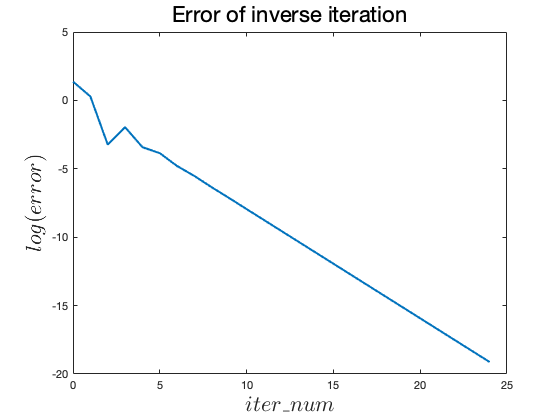
\includegraphics[width=0.5\linewidth]{code/inv_iter}
    	\caption{}
    	\label{fig:inviter}
    \end{figure}
    \begin{figure}
    	\centering
    	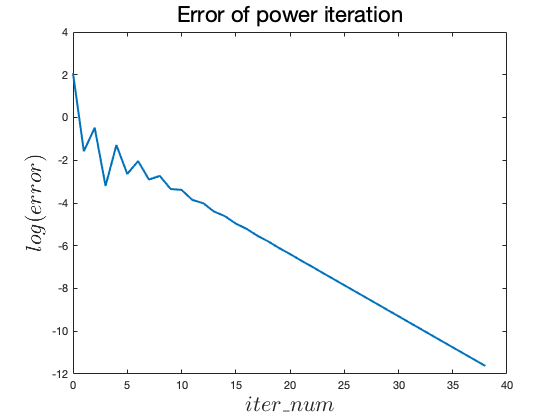
\includegraphics[width=0.5\linewidth]{code/power_iter}
    	\caption{}
    	\label{fig:poweriter}
    \end{figure}
set A as \[
\bA = \begin{bmatrix}
	0 & 4.6 \\
	3.4 & 0
\end{bmatrix}\,,\quad \text{ with }\alpha,\beta > 0\,.
\]
Both of the above methods can converge .You can see figure 1 and figure 2.

Some analysis:\\
\begin{enumerate}
	\item $
	v_{0}=\alpha_{1} x_{1}+\alpha_{2} x_{2}+\cdots+\alpha_{n} x_{n} \quad\left(\alpha_{1} \neq 0\right) \\$
	$
	v_{1}=A v_{0}=\alpha_{1} \lambda_{1} x_{1}+\alpha_{2} \lambda_{2} x_{2}+\cdots+\alpha_{n} \lambda_{n} x_{n}$\\
	$
	\begin{aligned}
		v_{k} &=A v_{k-1}=\alpha_{1} \lambda_{1}^{k} x_{1}+\alpha_{2} \lambda_{2}^{k} x_{2}+\cdots+\alpha_{n} \lambda_{n}^{k} x_{n} \\
		&=\lambda_{1}^{k}\left[\alpha_{1} x_{1}+\alpha_{2}\left(\frac{\lambda_{2}}{\lambda_{1}}\right)^{k} x_{2}+\cdots+\alpha_{n}\left(\frac{\lambda_{n}}{\lambda_{1}}\right)^{k} x_{n}\right]
	\end{aligned}
	$
	
	
	The smaller the value of $|\frac{\lambda_1}{\lambda_2}|$, the faster the convergence will come. If the absolute value of the two eigenvalues is the same, then it will not converge. If the eigenvalue difference is relatively small, the convergence will be very slow.
	
	For example:
	
	set A as \[
	\bA = \begin{bmatrix}
		0 & 5 \\
		1 & 0
	\end{bmatrix}
	\]
	$\lambda_1 = 2.23$ $\lambda_2 = -2.23$ 
	\begin{figure}
		\centering
		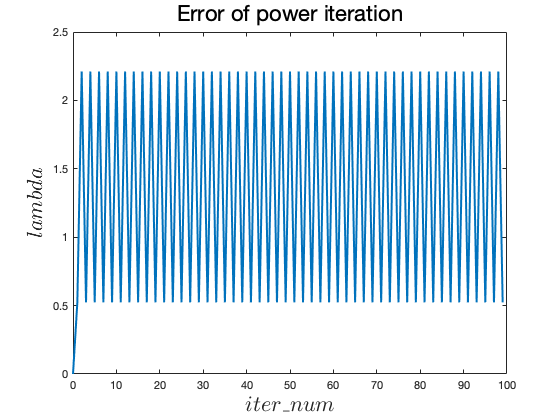
\includegraphics[width=0.5\linewidth]{code/power_iter_not}
		\caption{}
		\label{fig:poweriternot}
	\end{figure}
	Iteration cannot converge, as you can see in figure 3.
	
	\item For the inverse power method, mu should not be placed in the middle of the two eigenvalues.
	
	set A as \[
	\bA = \begin{bmatrix}
		0 & 5 \\
		1 & 0
	\end{bmatrix}\,
	\]
	$\lambda_1 = 2.23$ $\lambda_2 = -2.23, mu = 0$  
	Iteration cannot converge, as you can see in figure 4.
	\begin{figure}
		\centering
		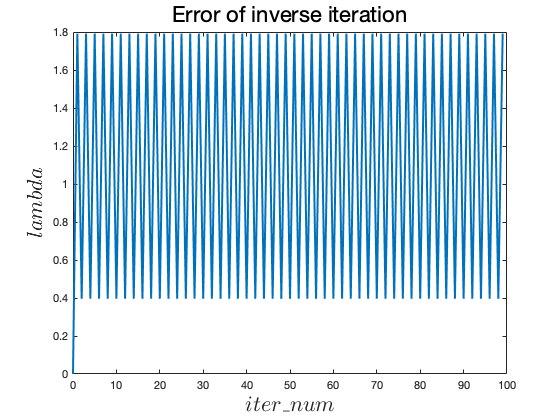
\includegraphics[width=0.5\linewidth]{code/inv_iter_not}
		\caption{}
		\label{fig:inviternot}
	\end{figure}
	
\end{enumerate}




\end{enumerate}


\newpage 
\subsection{QR itertiaon and Hessenberg QR iteration}
\noindent
\textbf{Recap.}
For $\bA \in \mathbb{C}^{n\times n}$,
consider the QR iteration (See Algorithm \ref{alg:qr_iter}) for finding all the eigenvalues and eigenvectors of $\bA$. 
\begin{algorithm}[htbp]
	\label{alg:qr_iter}
	\SetKwInOut{Input}{Input}\SetKwInOut{Output}{Output}
	\caption{QR iteration}
	\SetAlgoLined
	\Input{$\bA \in \mathbb{C}^{n\times n}$}
	\textbf{Initilization:} $\bA^{(0)} = \bA$.\\
	\For{$k= 1,\ldots, $}{
		$\bQ^{(k)}\bR^{(k)} = \bA^{(k-1)}$ \textcolor{blue}{\texttt{ \% Perform QR for $\bA^{(k-1)}$}}\\
		$\bA^{(k)} = \bR^{(k)}\bQ^{(k)}$
	}
	\Output{$\bA^{(k)}$}
\end{algorithm}
In each iteration, $\bA^{(k)}$ is similar to $\bA$ in that 
\begin{align*}
 	\bA^{(k)}
 	&  = \bR^{(k)}\bQ^{(k)} = (\bQ^{(k)})^H \bQ^{(k)}\bR^{(k)}\bQ^{(k)} = (\bQ^{(k)})^H \bA^{(k-1)}\bQ^{(k)}= \cdots \\
 	& = (\bQ^{(1)}\bQ^{(2)} \cdots \bQ^{(k)})^H \bA (\bQ^{(1)}\bQ^{(2)} \cdots \bQ^{(k)})  \Rightarrow \bA^{(k)} \text{ is similar to } \bA\,.
\end{align*}
Suppose the Schur decomposition of $\bA$ is $\bA = \bU \bT \bU^H$, then under some mild assumptions, $\bA^{(k)}$ converges to $\bT$.
Therefore, we can compute all the eigenvalues of $\bA$ by taking the diagonal elements of $\bA^{(k)}$ for sufficiently large $k$.
However, each iteration requires $\bigO(n^3)$ flops to compute QR factorization which is computationally expensive.
\begin{algorithm}[htbp]
	\label{alg:hessen_qr_iter}
	\SetKwInOut{Input}{Input}\SetKwInOut{Output}{Output}
	\caption{Hessenberg QR iteration}
	\SetAlgoLined
	\Input{$\bA \in \mathbb{C}^{n\times n}$}
	\textbf{Initilization:} $\bH = \bQ^H \bA \bQ\,,\bA^{(0)} = \bH$.  \textcolor{blue}{\texttt{ \% Hessenberg reduction for $\bA$}}\\
	\For{$k= 1,\ldots, $}{
		$\bQ^{(k)}\bR^{(k)} = \bA^{(k-1)}$ \textcolor{blue}{\texttt{ \% Perform QR for $\bA^{(k-1)}$ using Givens QR}}\\
		$\bA^{(k)} = \bR^{(k)}\bQ^{(k)}$ \textcolor{blue}{\texttt{ \% Matrix computation}}
	}
	\Output{$\bA^{(k)}$}
\end{algorithm}
One possible solution is: first perform similarity transform $\bA$ to an upper Hessenberg form (Step 1 in Algorithm \ref{alg:hessen_qr_iter}), then perform QR iteration (Algorithm \ref{alg:qr_iter}) over new $\bA^{(0)} = \bH$.
By using Givens rotations, the QR step only takes $\bigO(n^2)$ flops. 

\clearpage
\textbf{Problem 6.}
\textcolor{blue}{(15 points +10 points)}

\noindent
\begin{enumerate}
    \item Complete the Algorithm \ref{alg:hessen_qr_step} (corresponding to the step 3-4 of Algrorithm \ref{alg:hessen_qr_iter} ) first \textcolor{blue}{(7 points)}, then
show \textbf{the detailed derivation} of the computational complexity of in Algorithm \ref{alg:hessen_qr_step} ($\bigO(n^2)$). \textcolor{blue}{(8 points)}
(Derivation is for the computaional complexity of the algorithm.)

To be more specific, we can present the process of performing QR for $\bA^{(k)}$ using Givens rotations as:
\begin{enumerate}
\item[(a)] First, overwrite $\bA^{(k)}$ with upper-triangular $\bR^{(k)}$
\[
\bA^{(k)} = (\bG_{m}^H \bG_{m-1}^H \cdots \bG_{1}^H) \bA^{(k)} = \bR^{(k)}\,,
\]
where $\bG_{1},\ldots,\bG_{m}$ is a sequence of Givens rotations for some $m$ (In your algorithm, you need to clearly specify what $\bG_i$ is), and $\bR^{(k)}=\bG_1 \cdots \bG_{m}$.
\item[(b)] Perform matrix multiplication such that $\bA^{(k)}$ is of Hessenberg form,
\[
\bA^{(k)} = \bR^{(k)}\bQ^{(k)} = \bA^{(k)}\bG_1 \cdots \bG_{m}\,.
\]
\end{enumerate}
\item 
\textcolor{blue}{\textbf{(Bouns Problem})}
\textbf{Implicit QR iteration}

Another way to implement step 3-4 in Algorithm \ref{alg:hessen_qr_iter} is through \textit{implicit QR iteration}.
The idea is as follows, for $\bA^{(0)}\in \mathbb{R}^{n\times n}$ which is of Hessenberg form,
\begin{enumerate}
    \item[(a)] First, compute a Givens rotation $\bG_1$ such that $(\bG_1^{H}\bA^{(0)})_{2,1} =0$ and update $\bA^{(1)}  = \bG_1^{H} \bA^{(0)} \bG_1$. However, the entry $\bA^{(1)}_{3,1}$ may be nonzero (known as "bulge").
    \item[(b)] Compute another Givens rotation $\bG_2$ such that $(\bG_2\bA^{(1)})_{3,1} =0 $ (i.e., nulling out the "bulge") and update $\bA^{(2)}  = \bG_2^{H} \bA^{(1)} \bG_2$ which is analogous with step (a). Note that the entry $\bA^{(2)}_{4,2}$ will now be nonzero.
    \item[(c)] Then, we try to find $\bG_3$ such that $(\bG_3\bA^{(2)})_{4,2}=0$.
    The procedure of iterating nulling out the "bulges" to reset in a upper Hessenberg form is known as "bulge chasing".
\end{enumerate}
This algorithm \textit{implicitly} computed QR factorization at the cost of $\bigO(n^2)$, and this is why the algorithm is called the \textit{Implicit QR iteration}.
Consider a $4\times 4$ Hessenberg matrix
\[
\bA^{(0)} = \begin{bmatrix}
       1 & 2 & 3 & 4\\
       2 & 3 & 1 & 2\\
       0 & 1 & 3 & 2 \\
       0 & 0 & 2& 1
\end{bmatrix}\,.
\]
Carry out the implicit QR iteration (show the detailed derivation) (To simplify the computation, you can use \codeword{Matlab} to do the matrix multiplications. Specifically, explicitly show $\bG_i$, $\bG_i^H\bA^{(i-1)}$ and $\bA^{(i)}$ for each step but when computing the matrix multiplication such as $\bG_i^H\bA^{(i-1)}$, $\bG_i^H\bA^{(i-1)}\bG_i$, you are free to use \codeword{Matlab}. But be careful with the precision issue during the process of computing.), and observe where does the so-called "bulge" appears. \textcolor{blue}{(5 points: including the detailed derivation of the implicit QR iteration and pointing out the "bulge")}
Based on your observations, explain why the implicit QR iteration is indeed equivalent to the Algorithm \ref{alg:hessen_qr_step}. \textcolor{blue}{(5 points)}
\end{enumerate}




\begin{algorithm}[htbp]
	\label{alg:hessen_qr_step}
	\SetKwInOut{Input}{Input}\SetKwInOut{Output}{Output}
	\caption{Step 3-4 in Hessenberg QR iteration}
	\SetAlgoLined
	\Input{$\bA^{(k-1)} \in \mathbb{C}^{n\times n}$ which is of upper Hessenberg form \textcolor{blue}{\texttt{ \% corresponding to $\bA^{(k-1)}$ in step 3 of Algorithm \ref{alg:hessen_qr_iter}}}} 
	\textcolor{blue}{\texttt{ \% Perform QR for $\bA^{(k)}$ using Givens roations}}\\
		\For{$k= 1: n-1$}{
			$\bA(k: k+1, k: n)=\left[\begin{array}{rr}
				c_{k} & s_{k} \\
				-s_{k} & c_{k}
			\end{array}\right]^{T} \bA(k: k+1, k: n)$\\
		
	}
	\textcolor{blue}{\texttt{ \% Matrix computation}}\\
	\For{$k= 1: n-1$}{
		$H(1: k+1, k: k+1)=H(1: k+1, k: k+1)\left[\begin{array}{rr}
			c_{k} & s_{k} \\
			-s_{k} & c_{k}
		\end{array}\right]$\\
	}

	\Output{$\bA^{(k)}$ \textcolor{blue}{\texttt{ \% corresponding to $\bA^{(k)}$ in step 4 of Algorithm \ref{alg:hessen_qr_iter}}}}
\end{algorithm}





\noindent
\textbf{Solution}
\begin{enumerate}
    \item[1.(b)] Perform matrix multiplication such that $\bA^{(k)}$ is of Hessenberg form, Every time we perform householder transformation, we only need to eliminate the elements of the diagonal line one by one.
    
    Assuming that A has n rows, then it needs to be eliminated n-1 times given elimination
    
    Every Givens elimination we multiplies A by $2 \times 2$ rotation matrix, we need to caculate the rotation matrix as following:
    
    
    $Q = I-2vv^T$, $v = ||a_i||_2-a_i$, $v = \frac{v}{||v||_2}.$  it costs const flops.
    
    1. rotation matrix cost 10 flops.
    
    2.$\left[\begin{array}{rr}
    	c_{k} & s_{k} \\
    	-s_{k} & c_{k}
    \end{array}\right]^T \bA(k: k+1, k: n)$ cost n flops,as data is accessed across rows

   3.$H(1: k+1, k: k+1)\left[\begin{array}{rr}
   	c_{k} & s_{k} \\
   	-s_{k} & c_{k}
   \end{array}\right]$cost n flops,as data is accessed across rows

	All in all total cost is $n*(10 + n + c) + n*n.$  so is $\bigO(n^2)$
    \item[2.]
    
\end{enumerate}

\end{document}